\documentclass{article}
\usepackage{tikz}
\usepackage{pgf-umlcd}
\begin{document}
%\section*{Clase abstracta Empleado}
%\begin{center}
%\begin{tikzpicture}
%  \begin{class}[text width=8cm]{Empleado}{0,0}
%    \attribute{nombre : string}
%    \attribute{domicilio : string}
%    \attribute{numeroSeguridadSocial : string}
%    \attribute{fechaContratacion : string}
%    \attribute{salario : f\/loat}
%    
%    %\operation{name(parameter list) : type of value returned}
%    % virtual operations
%    %\operation[0]{name(parameters list) : type of value returned}
%    \operation[0]{calcularSalario() : void}
%  \end{class}
%\end{tikzpicture}
%\end{center}
%\section*{Clase abstracta FiguraGeometrica}
%\begin{center}
%\begin{tikzpicture}
%  \begin{class}[text width=8cm]{FiguraGeometrica}{0,0}
%    \attribute{area : f\/loat}
%    %\attribute{domicilio : string}
%    %\attribute{numeroSeguridadSocial : string}
%    %\attribute{fechaContratacion : string}
%    %\attribute{salario : f\/loat}
%    
%    %\operation{name(parameter list) : type of value returned}
%    % virtual operations
%    %\operation[0]{name(parameters list) : type of value returned}
%    \operation[0]{calcularArea() : void}
%  \end{class}
%\end{tikzpicture}
%\end{center}
\section*{Clase DFecha}
\begin{center}
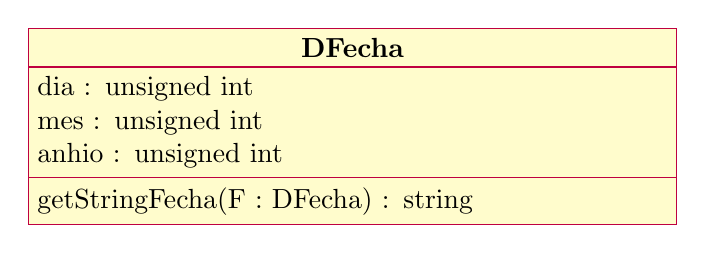
\begin{tikzpicture}
  \begin{class}[text width=8cm]{DFecha}{0,0}
    \attribute{dia : unsigned int}
    \attribute{mes : unsigned int}
    \attribute{anhio : unsigned int}
    %\attribute{fechaContratacion : string}
    %\attribute{salario : f\/loat}
    
    \operation{getStringFecha(F : DFecha) : string}
    % virtual operations
    %\operation[0]{name(parameters list) : type of value returned}
    %\operation[0]{calcularArea() : void}
  \end{class}
\end{tikzpicture}
\end{center}
\begin{verbatim}
/**DFecha.h
 */
struct Fecha{
  unsigned int d,m,a;  /*dia,mes,an\~{n}o*/
};/*end struct Fecha*/
string get_string_fecha(struct Fecha F);
\end{verbatim}
\end{document}